% TODO JAMES where to write more? bg/theory, diagrams/examples
% TODO JAMES is "classification accuracy" correct?
% TODO JAMES good idea to explain repo structure?


%TODO NOW rename slice optimisation


% TODO compare with other approaches (matern kernel)
% TODO don't stop time spent scoring
% TODO roc_auc_score to score
% TODO convert sparse arff files to non sparse
% TODO rnd forest is bad at data thats heavily pos or neg
% TODO describe gradent problems
% TODO describe classifier scoring mechanism
% TODO optimisation: gpml's didn't work, rolled my own based on slice optimisation; explain grad based optimi, show nlml func to justify that it's simple
% TODO implement better optimiser based on gradients
% TODO comparing model evidence
% TODO look at spearmint
% TODO Nearest Neighbors Classification
% TODO describe ranges
% TODO figure/Figure capitalisation
% TODO present/past
% TODO UML diagram for schedulers
% TODO If you use purely-numeric bibliographic references, do not forget to still mention authors’ surnames
% TODO describe kernel problems
% TODO establish the words scheduler and approx params early on
% TODO no emotional language
% TODO datasets: http://rodrigob.github.io/are_we_there_yet/build/classification_datasets_results.html
% TODO explain datasets w/ images if they are interesting
% TODO explain repo directory structure
% TODO stress that the gradients are correct

% TODO Where a project has as its main aim the production of a piece of software, the project report should state clearly what test procedures were adopted and should include test output


% TODO Datasets
%- Autoweka data taken from their website (how were those datasets selected?)
%- merge training and test arffs using weka cmd line
%python:
%- load using scipy.io.arff.loadarff
%- vectorise (one-of-K) using sklearn.feature_extraction.DictVectorizer

\documentclass[a4paper,12pt,twoside,openright]{report}

% Diagrams
\usepackage{graphicx}

\def\authorname{Jan S\"ondermann\xspace}
\def\authorcollege{Selwyn College\xspace}
\def\authoremail{jjes2@cam.ac.uk}
\def\dissertationtitle{Bayesian optimisation of approximateness in the trade-off between statistical and computational efficiency}
% TODO word count
\def\wordcount{@}

\usepackage{subcaption}
\usepackage{chngpage}
\usepackage{calc}
\usepackage{epsfig,graphicx,parskip,setspace,tabularx,xspace} 
\usepackage{enumitem}
\usepackage{mathtools}
\usepackage{amsmath,amssymb}
\usepackage{algorithmicx}
\usepackage{algorithm}% http://ctan.org/pkg/algorithms
\usepackage{algpseudocode}
\newcommand{\Break}{\State \textbf{break} }

% Source code listings
\usepackage{listings}
\lstset{breaklines=true, frame=single, numbers=left, basicstyle=\small\ttfamily}

% TODO make this work
%\lstset{ %
%  commentstyle=\color{grey}    % comment style
%}


%% START OF DOCUMENT
\begin{document}


%% FRONTMATTER (TITLE PAGE, DECLARATION, ABSTRACT, ETC) 
\pagestyle{empty}
\singlespacing
% title page information
\begin{titlepage} 

\begin{center}
\noindent
\huge
\dissertationtitle \\
\vspace*{\stretch{1}}
\end{center}

\begin{center}
\noindent
\huge
\authorname \\
\Large
\authorcollege      \\[24pt]

\includegraphics{CUni3.eps}
\end{center}

\vspace{24pt} 

\begin{center}
\noindent
\large
{\it A dissertation submitted to the University of Cambridge \\ 
in partial fulfilment of the requirements for the degree of \\ 
Master of Philosophy in Advanced Computer Science} 
\vspace*{\stretch{1}}
\end{center}

\begin{center}
\noindent
University of Cambridge \\
Computer Laboratory     \\
William Gates Building  \\
15 JJ Thomson Avenue    \\
Cambridge CB3 0FD       \\
{\sc United Kingdom}    \\
\end{center}

\begin{center}
\noindent
Email: \authoremail \\
\end{center}

\begin{center}
\noindent
\today
\end{center}

\end{titlepage} 

\newpage
\vspace*{\fill}

\onehalfspacing
\newpage
{\Huge \bf Declaration}

\vspace{24pt} 

I \authorname of \authorcollege, being a candidate for the M.Phil in
Advanced Computer Science, hereby declare that this report and the
work described in it are my own work, unaided except as may be
specified below, and that the report does not contain material that
has already been used to any substantial extent for a comparable
purpose.

\vspace{24pt}
Total word count: \wordcount

\vspace{60pt}
\textbf{Signed}: 

\vspace{12pt}
\textbf{Date}:


\vfill

This dissertation is copyright \copyright 2010 \authorname. 
\\
All trademarks used in this dissertation are hereby acknowledged.



\newpage
\vspace*{\fill}

\singlespacing
\newpage
{\Huge \bf Abstract}
\vspace{24pt} 


% TODO write abstract
%Our project falls into the field of meta-machine learning that tries to use machine learning methods to improve the result of using these methods.


\newpage
\vspace*{\fill}


\pagenumbering{roman}
\setcounter{page}{0}
\pagestyle{plain}
\tableofcontents
\listoffigures
\listoftables

\onehalfspacing

%% START OF MAIN TEXT 

\chapter{Introduction}
\pagenumbering{arabic} 
\setcounter{page}{1} 

- context
- motivation
- general overview
% TODO context (why did you do it (motivation), what was the hoped-for outcome (aims) --- as well as trying to give a brief overview of what you actually did)


% TODO It's often useful to bring forward some ``highlights'' into  this chapter (e.g.\ some particularly compelling results, or  a particularly interesting finding). 

% TODO It's also traditional to give an outline of the rest of the document, although without care this can appear formulaic and tedious. Your call. 


\chapter{Background}
% TODO The report should explicitly describe the starting point for the project, making clear what existing software or other resources were used
\section{Data sources}
%- explain where the data came from and how it was preprocessed

% TODO mention: sklearn, gpml, jsonlab

\textit{This chapter describes the background assumed in the remainder of the document. Specifically, it }
\section{Machine Learning}
\section{Algorithms}
\subsection{Gaussian Processes}
\subsection{Random Forests and Logistic Regression}

% TODO explain hyperparameters
%as this is meta machine learning, i have to introduce @normal machine learning at a high level@
%algos + their imple (rf, lr, gps)


%- GPs/GPML (marginal likelihood)


% describe scheduling

% TODO A more extensive coverage of what's required to understand your work. In general you should assume the reader has a good undergraduate degree in computer science, but is not necessarily an expert in the particular area you've been working on. Hence this chapter may need to summarise some ``text book'' material. 



\chapter{Related Work} 

%- hyper param optim
%- multi armed bandits

% TODO This chapter covers relevant (and typically, recent) research which you build upon (or improve upon). There are two complementary goals for this chapter: - to show that you know and understand the state of the art; and to put your work in context

% TODO Ideally you can tackle both together by providing a critique of related work, and describing what is insufficient (and how you do better!)







% TODO "classification accuracy" maybe isn't correct if we also use roc
% TODO mention somewhere that "performance" means time + score
\chapter{Design and Implementation} 



\textit{This chapter describes the theoretical and practical aspects system we developed. It firsts gives a high level overview of the system architecture before describing in detail the two main parts of the program: modelling performance and scheduling.}

\section{Architecture} % TODO maybe something like "overview"
\subsection{Key concepts}
\subsubsection{Approximation parameters}
Approximation parameters are parameters to the machine learning algorithms that influence the trade-off between statistical and computational efficiency. They let us vary the degree of approximateness at which the algorithm runs. Changing an approximation parameters should either decrease the run time at the cost of classification accuracy or improve accuracy while making training slower. 

The approximation parameter that we put most of our focus on in this project is the proportion of the available data. Other approximation parameters are hyperparameters to the machine learning algorithms such as the number of decision trees in a random forest. No all hyperparameters, however, are approximation parameters. Examples of hyperparameters that have no influence on performance are the lengthscale of a kernel and the 
% TODO mention parameters like #thread that influence time but not performance
@not all hyps are appr.(length scale). always distinguish between two@

\subsubsection{Scheduling}


\subsection{High level architecture}
% TODO END make sure this is properly centered
\begin{figure}[!ht]
  \begin{adjustwidth}{-\oddsidemargin-2in}{-\rightmargin-1.5in}
    \centering
    \includegraphics[trim=0 0 0 0,clip,width=0.9\paperwidth]{figures/architecture.pdf}
    
  \end{adjustwidth}
  \caption{High level architecture, shown after three iterations. Data is coloured red, machine learning algorithms are coloured blue}
    \label{architecture}
\end{figure}

Our system is designed in a two tiered fashion. Tier 1 creates models of the data using learning algorithms that are parameterised with approximation parameters. The training time and prediction accuracy of these models makes up the input to tier 2. This second layer first creates a meta-model of the model performances of the models in tier 1. This meta-model is then used by the scheduling part of the program to select the algorithm and approximation parameters for the next iteration. 

Figure \ref{architecture} shows this architecture diagrammatically after three iterations. Note how both tiers execute machine learning algorithms (coloured in blue) on a set of data (coloured in red) and how the result of the algorithms in the first tier form the data set for the Gaussian Process at the top of the diagram. The main loop of our program is shown, slightly simplified, in Figure \ref{mainloop}. When executing, the program switches back and forth between the two tiers: it executes an algorithm with a given set of approximation parameters, builds a new model that includes the performance during this execution. The scheduler then decides which algorithm/approximation parameter combination to run next and the system returns to the first step.

\begin{figure}[ht]
\begin{lstlisting}[language=Python]
while True:
   scheduler.decide() # Tier 2 (scheduling)
   if scheduler.decision:
      scheduler.execute() # Tier 1
      scheduler.model() # Tier 2 (modelling)
\end{lstlisting}
\caption{The main loop}
\label{mainloop}
\end{figure}

% TODO tier 1 is standard ml stuff (using sklearn), our contribution is tier 2, has two parts: modelling and scheduling, now describe in detail




\section{Tier 1}
This section will @explain details@ of tier 1 before @moving on@ to tier 2 where out main contributions lie in the rest of this chapter.
% TODO mention k fold
% TODO roc (only used for binary, is valid as no comparison between binary and non binary

\section{Modelling Model Performance}
To make good decisions, the scheduler needs an accurate model of the dependance of approximation parameters and performance. Creating such models is therefore a fundamental piece in our system.

\subsection{Data Collection}
The first step towards modelling performance was to collect sample data. This data was used to first investigate the function and formulate a hypothesis on the character of the function from approximation parameters to performance. After the kernel was implemented, we tested it by comparing its predictions based on the sample data with possible alternative kernels. The details of this are described in the Evaluation chapter below.

% TODO MAYBE don't call this a script
\subsubsection{Data collection script}
As data collection was resource and time intensive, we implemented a command line script that accepts a range of configuration flags and collects data based on the parameters it receives. This script was then executed on an Amazon EC2 instance. This script can be configured with the following list of command line flags:

\begin{itemize}
\item \texttt{-a/--algorithm} The machine learning algorithm to be run. This can be one of \texttt{rnd\_forest}, \texttt{log\_reg} or \texttt{svm}
\item Exactly one out of the following ways to load data:
\begin{itemize}[label=$\star$]
        \item \texttt{-s/--synthetic} Create synthetic data using scikit-learn's \texttt{make\_classification}. The parameters to \texttt{make\_classification} should be specified in string containing a python dictionary (e.g. \texttt{"{'n\_samples': 5000}"})
        \item \texttt{-l/--load-arff} Load one of the \texttt{arff} files in the \texttt{data} directory
        \item \texttt{-z/--datasets-of-size} This loads all the datasets of the given size. Can be one of \texttt{small}, \texttt{medium} or \texttt{large}
        \item Vector Space Models
     \end{itemize}
\item \texttt{-d/--percentage-data-values} An array of data percentages specified in the syntax explained below
\item Any additional parameters in the form \texttt{parameter\_name:[int|float]-<array of values as explained below>}
\item \texttt{-p/--parallel} This flag was originally included to parallelise data collection by using multiple threads. Testing it revealed that running multiple instances of the algorithms in parallel led to distorted running times. This flag was not used for data collection
\end{itemize}

% TODO are these really sequences?
The syntax to specify arrays in the command line arguments allows expressing arithmetic and geometric sequences. Arithmetic sequences are created with \texttt{a:min:length:max}, e.g. \texttt{a:1:4:50} to create an array of four evenly spaced elements with the first being 1 and the last being 50. The syntax to create geometric sequences is \texttt{g:min:length:max:base}. It includes the base of the geometric sequence. In this syntax, the array \texttt{[2, 4, 8, 16, 32, 64]} is expressed as \texttt{g:2:6:64:2}.

Avoiding hard coded values for data generation made it possible to quickly collect fresh data.
	




\texttt{Collected sample data}

% TODO JAMES maybe use different figures
\begin{figure}
\centering
  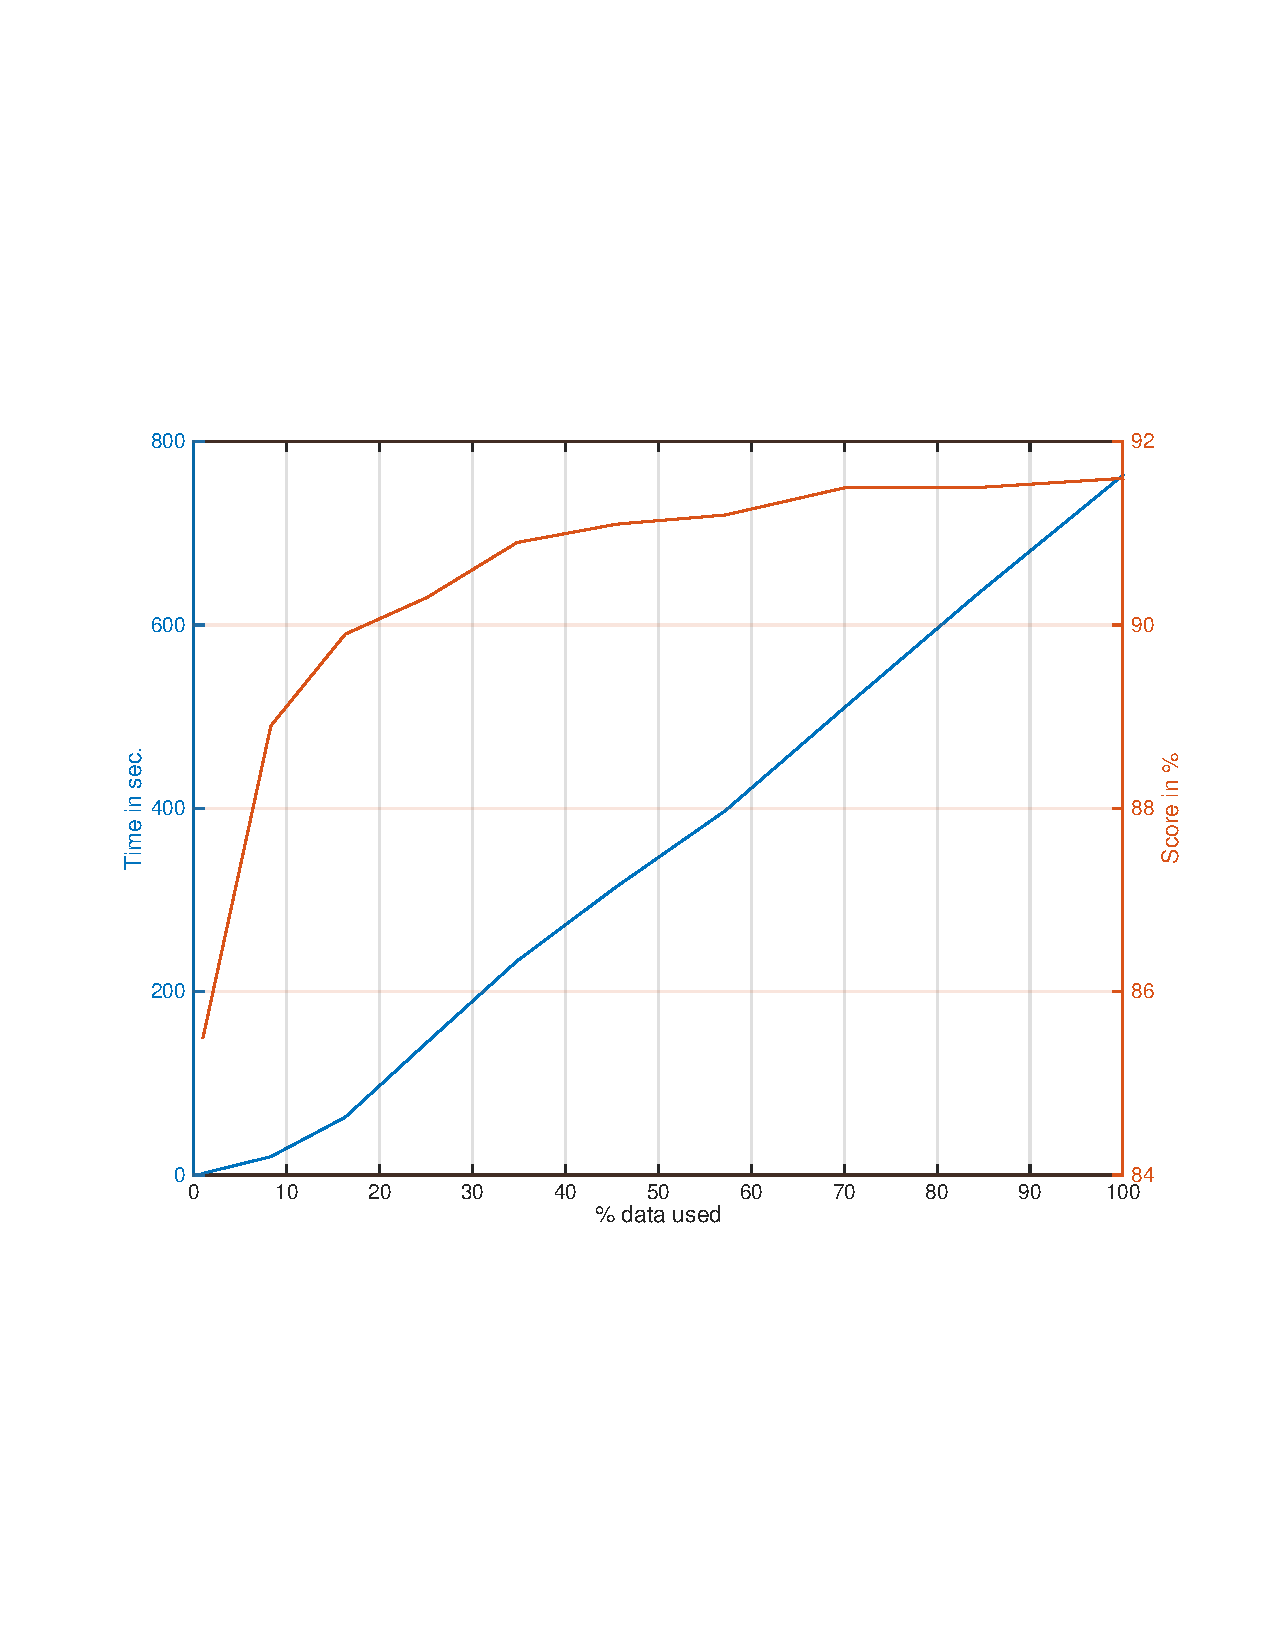
\includegraphics[trim=50 200 35 205,clip,width=.6\linewidth]{figures/lr_mnist.pdf}
  \caption{Running logistic regression on the MNIST dataset}
  \label{sampledata1}
\end{figure}

\begin{figure}
\centering
  \includegraphics[trim=50 200 35 205,clip,width=.6\linewidth]{figures/rf_mnist.pdf}
  \caption{Running random forest on the MNIST dataset}
  \label{sampledata2}
\end{figure}

\begin{figure}
\centering
  \includegraphics[trim=50 200 35 205,clip,width=.6\linewidth]{figures/lr_synth.pdf}
  \caption{Running logistic regression on a synthetic dataset}
  \label{sampledata3}
\end{figure}

\begin{figure}
\centering
  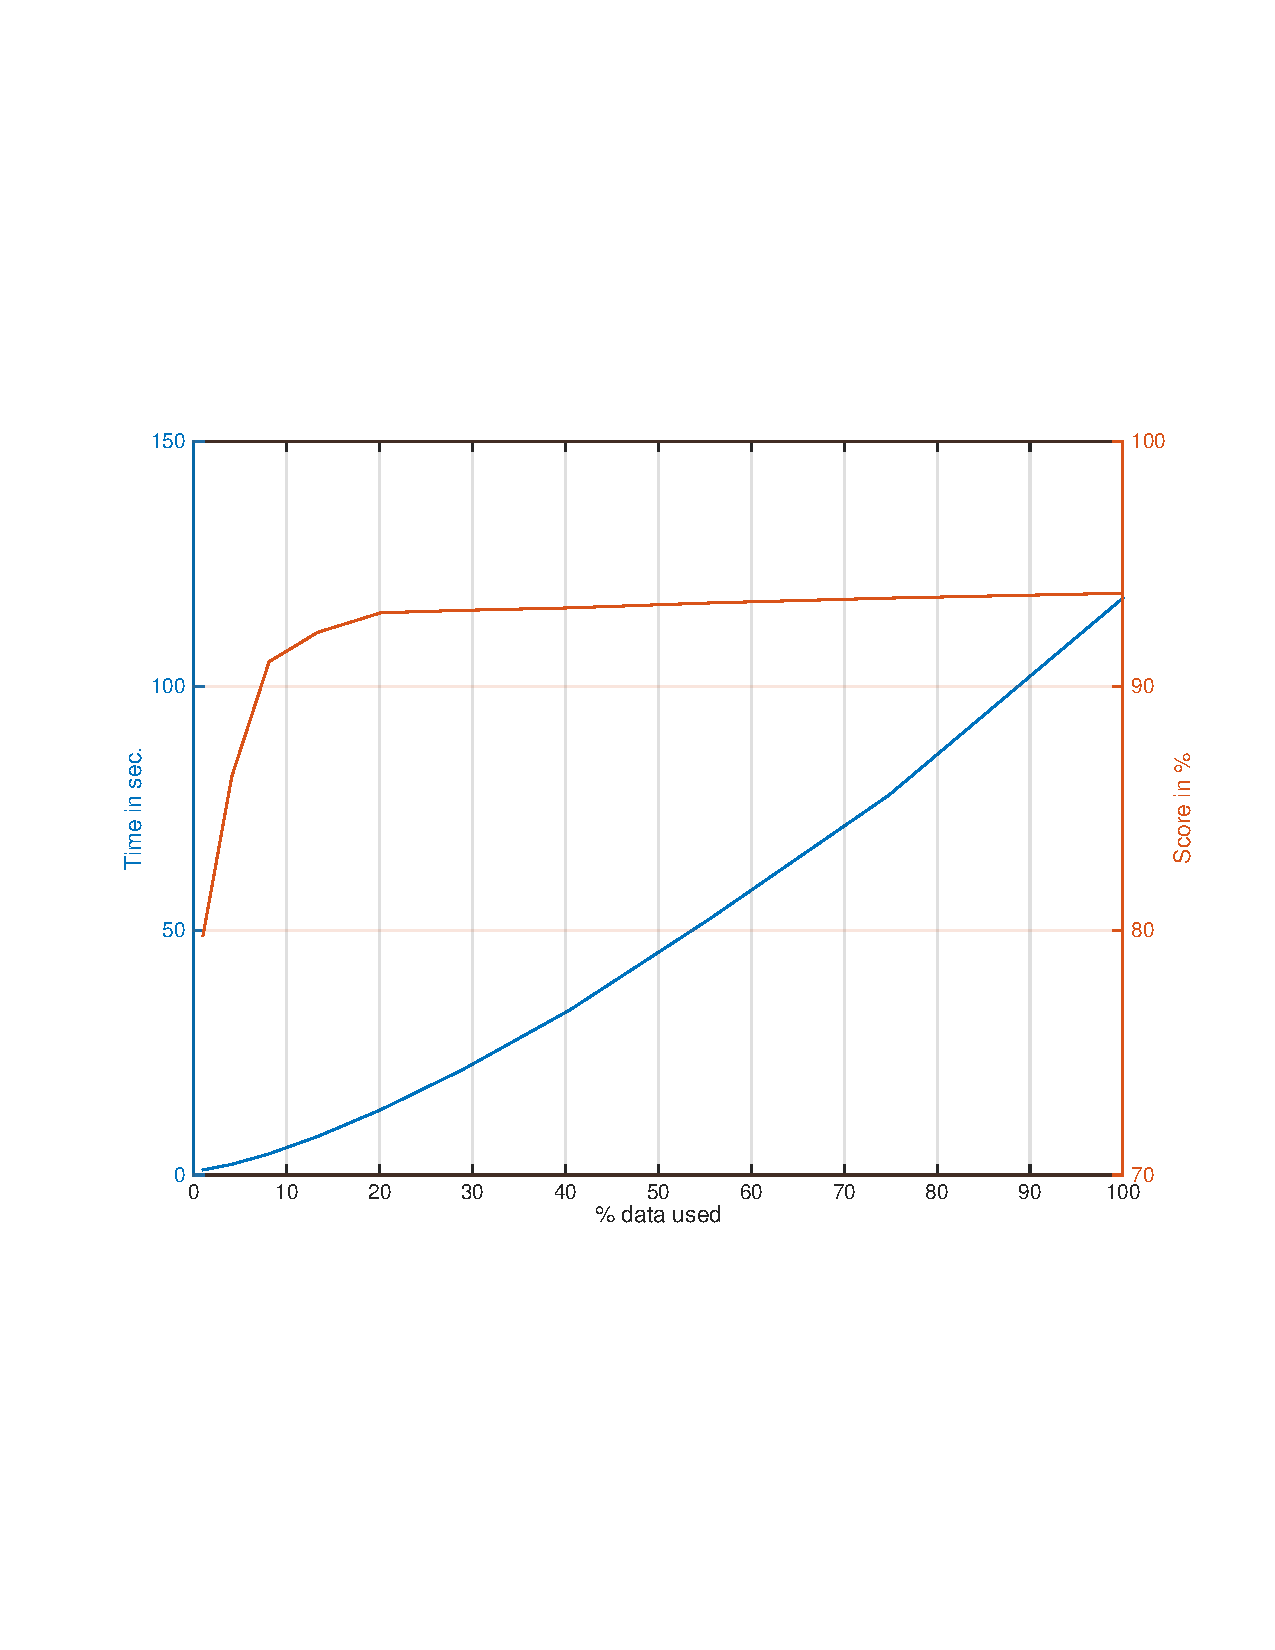
\includegraphics[trim=50 200 35 205,clip,width=.6\linewidth]{figures/rf_synth.pdf}
  \caption{Running random forest on a synthetic dataset}
  \label{sampledata4}
\end{figure}



% TODO why suddenly misclassification instead of accuracy, explain that one is 1-the other
Figures \ref{sampledata1}, \ref{sampledata2}, \ref{sampledata3} and \ref{sampledata4} show the results of collecting performance data, varying the percentage of data used. The four plots were generated by using random forest with 128 trees and logistic regression on the MNIST dataset and a synthetic dataset with 5000 samples and 500 features.

%how time (shown in @@) and misclassification rate (shown in @@) vary as different proportions of the available data are used in different combinations of algorithms and datasets. 


% TODO why did you select the appr params you selected, later you only use data. data is enough to be interesting but we want to show that approach can in principle be extended
% TODO look of O runtime of algos, should confirm empirical findings






\subsection{Exponential mixture kernel}
Based on the results shown in the previous section, we implemented a kernel to model the exponential behaviour of classification accuracy. Following \cite{2014arXiv1406.3896S}, we define the kernel as
% TODO JAMES can this be written as \psi(\lambda)d\lambda ?
\begin{align}
k(t,t') &= \int_{0}^{\infty} e^{-\lambda t}e^{-\lambda t'}\mu(d\lambda)\\
&= \int_{0}^{\infty} e^{-\lambda(t+t')}\mu(d\lambda)
\end{align}

% TODO kernel assumptions: decay starts at zero, maybe add limes
with $\mu$ being a mixing measure\footnote{We use $\mu$ instead of $\psi$ to denote the mixing measure to avoid confusion with the $\psi$ parameter to the gamma function explained below.}that weighs the $e^{-\lambda(t+t')}$ term. Note that this is not a stationary kernel as $k(t, t') \neq k(a + t, a + t')$. This conforms to our prior that moving further away from the origin, the value of $k$ should decrease.

Again following \cite{2014arXiv1406.3896S}, we choose a gamma distribution as $\mu$ which leads to an analytic solution to the integral:
\begin{align}
k(t, t') &= \int_0^{\infty} e^{-\lambda(t+t')}\frac{\beta^\alpha}{\Gamma(\alpha)}\lambda^{\alpha -1}e^{-\lambda\beta} d\lambda\\
&=\frac{\beta^\alpha}{\Gamma(\alpha)}\int_0^\infty e^{-\lambda(t+t'+\beta)}\lambda^{\alpha-1}d\lambda\\
&=\frac{\beta^\alpha}{(t+t'+\beta)^\alpha}
\end{align}

Diverging from \cite{2014arXiv1406.3896S}, we reparameterise the gamma distribution with
\begin{equation}
\psi = \mathbb{E}(x) = \frac{\alpha}{\beta}
\end{equation}
and
\begin{align}
\xi &= \frac{Var(x)}{\mathbb{E}^2 (x)} = \frac{\alpha}{\beta^2} \cdot \frac{\beta^2}{\alpha^2}\\
&= \frac{1}{\alpha}
\end{align}

% TODO show plots of reparameterised gamma function
% TODO show plots drawn from priors



\subsection{Selecting Kernel Hyperparameters} 
% TODO JAMES is it correct to call this model selection?

To fit a Gaussian process to a given set of data points, one needs to find appropriate values for the hyperparameters to its covariance and likelihood function. There two main methods to achieve this are marginalisation and optimisation. For reasons explained in the evaluation chapter, we implement both of these methods in our project.

% TODO this algorithm is "too clever"
% TODO show figs where optimisation fails
GPML comes with an optimisation function that is meant to be used to optimise hyperparameters. It relies on gradient information which we implemented for the exponential mixture kernel. We were, however, not able to use this function with our kernel as it would terminate after a very small number of steps having barely moved from the initial values without having found a minimum. We suspect the reason for this to be numerical instability that creates very small local minima that the optimiser is unable to escape from. Figure @ shows an example of a marginal likelihood function that we tried to optimise with GPML's \texttt{minimize}.

After failing to optimise the hyperparameters to our kernel using the optimisation function included with GPML, we decided to implement sampling which does not suffer from the same problems as optimisation. For reasons of speed and ease of use, we then decided to implement our own optimisation routine which is described in detail below. An evaluation of the two methods applied to our data can be found in the Evaluation chapter.


\subsubsection{Sampling}
The first approach to hyperparameter selection we use in our project is the Bayesian approach of integrating out the hyperparameters $\theta$:
\begin{equation}
p(y|X) = \int p(y|X,\theta)p(\theta)d\theta
\end{equation}


We decided to implement slice sampling

decided to implement this when gpml minimise didn't work


%The Bayesian way to handle hyperparameters is to integrate them out. 
% TODO add maths on integrating out hyperparams

%To approximate this integral, MCMC methods are
% TODO maths on MCMC

%To sample from @ we use slice sampling. adv/disadv: \cite{neal2003}
% TODO why slice sampling and not another method
%- mcmc/sampling



\subsubsection{Optimisation}
Another approach to find suitable hyperparameters is to optimise the marginal likelihood of the model with respect to its hyperparameters. This has the advantage of being substantially faster than sampling. It is also easier to implement, as it returns one set of hyperparameters that can be used to make predictions instead of multiple samples that have to be correctly averaged over. The great disadvantage of optimisation is that it is prone to overfitting by choosing one optimum in cases where multiple viable optima exist. We describe situations in which we encountered this problem in the Evaluation chapter, comparing it with the results of slice sampling.



After inspecting the marginal likelihood function @of sample data@ in Matlab, we concluded that it is not a function that is inherently difficult to optimise and decided to implement our own optimisation routine. As we had already successfully sampled hyperparameters using slice sampling as described above, we implemented an optimisation method that works similarly to how slice sampling draws samples. The first version of this algorithm is shown below as Algorithm \ref{opti1}.


\begin{algorithm}
\begin{algorithmic}[1]
\Procedure{Slice\_optimisation}{$f,x,iterations=100,width=1$}
\State $y\gets f(x),\ D\gets \Call{get\_dimensions}{x}$
\For{$i\gets 1, iterations$}
\For{$dim\gets \Call{permute}{D}$}\Comment{Iterate over all dimensions}
\State $x_l, x_r, x'\gets x$\Comment{$x_l,\ x_r$ span interval, $x'$ falls inside}
\State $r\gets \Call{Uniform}{0, 1}$
\State $x_l(dim)\gets x(dim) - r * width$
\State $x_r(dim)\gets x(dim) + (1 - r) * width$
\For{$j\gets 1, 15$}
\State $x'(dim)\gets \Call{Uniform}{x_r(dim), x_l(dim)}$
\State $y' = f(x')$
\If{$y' < y$}
\State $y\gets y',\ x(dim) = x'(dim)$\Comment{New optimum}
\Break
\EndIf
\If{$x'(dim) > x(dim)$}
\State $x_r(dim) = x'(dim)$\Comment{Narrow interval from the right}
\ElsIf{$x'(dim < x(dim)$}
\State $x_l(dim) = x'(dim)$\Comment{Narrow interval from the left}
\EndIf
\EndFor
\EndFor
\EndFor
\EndProcedure
\end{algorithmic}
\caption{First version of slice optimisation}
\label{opti1}
\end{algorithm}

This optimisation algorithm starts at a given $x$ and optimises by iterating over the input dimensions, spanning up an interval around $x$ for every iteration. Inside of these iterations, it selects points $x'$ at random from the interval. If $f(x')$ is smaller than the current minimum, it continues to the next loop iteration, otherwise it narrows the interval either from the left or the right, depending on the side of $x$ on which $x'$ falls.

Given enough data, this algorithm is able to find suitable hyperparameters to the exponential mixture kernel reliably. If it is used to fit a GP to a small number of points (five or less), it often selects hyperparameters such that the covariance matrix is not positive semidefinite and Cholesky decomposition fails. We catch these errors by wrapping every evaluation of $f$ in a \texttt{try ... catch} block. 

While testing this algorithm, we found an effective method to handle these errors to be rerunning the algorithm multiple times and selecting the result with the highest marginal likelihood. This also alleviates the issue of local optima which we discuss in detail in the Evaluation chapter. The code to achieve this is shown as Algorithm \ref{optiwrap}.

\begin{algorithm}
\begin{algorithmic}[1]
\Procedure{Optimise\_with\_restarts}{$f,x,restarts=5$}
\State $X = [\ ],\ Y = [\ ]$
\For{$i\gets 1, restarts$}
\State $x'\gets \Call{Slice\_optimisation}{f, x}$
\State $y'\gets f(x')$
\State $\Call{append}{X, x'}$
\State $\Call{append}{Y, y'}$
\EndFor
\State $i\gets \Call{MinIndex}{Y}$
\State \textbf{return} $X(i)$
\EndProcedure
\end{algorithmic}
\caption{Rerunning the optimiser}
\label{optiwrap}
\end{algorithm}

While this updated algorithm produces adequate results, it takes a substantial amount of time to optimise. A final change we therefore added was to terminate the optimisation routine early if the value of $y$ only changes minimally between five optimisations. This condition is met during almost all iterations and often drastically cuts short the time that our algorithm needs.

% TODO MAYBE mention that there is an implementation of it, what did you try to make it work?
One shortcoming of this optimisation routine is that all its steps have to be axis aligned. If the gradient of the function being optimised at $x$ is not aligned with any axis, this causes the optimiser to make very small steps along multiple axes. A superior approach would be to directly move along the gradients, which are available to us. As our current algorithm already performs to a high standard, we did not investigate this potential improvement further.


% TODO mention that the result of optimisation is handled as one sample, averaged over one


%show diagrams, talk about the relationship. is it always linear for time (no, svm, O(n^2-3)), is it always exponential for score





\section{Scheduling} 

% TODO figures to explain different acquisition strategies

\chapter{Evaluation}
% TODO evaluate kernel (model evidence etc)
% TODO for 2d: plot variance
 
% TODO optimisation is faster and produces only one mean/sd, easier to use
% using the \texttt{checkgrad.m}
% compare optimisation/sampling adv/disadv
% TODO rasmussen: local maxima correspond to a particular interpretation of the data


\section{Results}

\subsection{Hyperparameter selection}


% TODO show case where one function is better initially but then gets overtaken
\section{Testing}
\section{Limitations}
\section{Challenges} % TODO most of this was prob mentioned in design&impl
% TODO numerical accuracy for EI when sd is very small and peak is under lower bound, i.e. prob of impr is very small, get infs and nans
%- model evidence
%- testing
%- how well it performs
% TODO "hinge" on my computer
% TODO kernel "cliffs"
% TODO optimisation gets overfits, too much confidence in one interpretation

\chapter{Conclusion and future work} 
\section{Conclusions}
\section{Future work}
% TODO additional appr params. the kernel is already implemented

% TODO Depending on the length of your work, and  how well you write, you may not need a summary here. You will generally want to draw some conclusions, and point to potential future work. 




\appendix
\singlespacing

\bibliographystyle{unsrt} 
\bibliography{references}


\end{document}
